\section{Regional Difference}

\subsection{USA}

\subsection{Japan}

Figure~\ref{fig:q5} shows the simple-tab results asking how many years
for writing programs (including MPI) and Figure~\ref{fig:q6} shows the
results asking how many years for writing MPI programs. Each bar
represents a country or region having more than 50 answers. ``whole''
represents the whole data and ``Europe:other'' represents the sum of
other European countries. The numbers
following the column titles represent the number of answers of that
country/region and the number of total answers of the question.

\begin{figure}[htb]
\begin{center}
  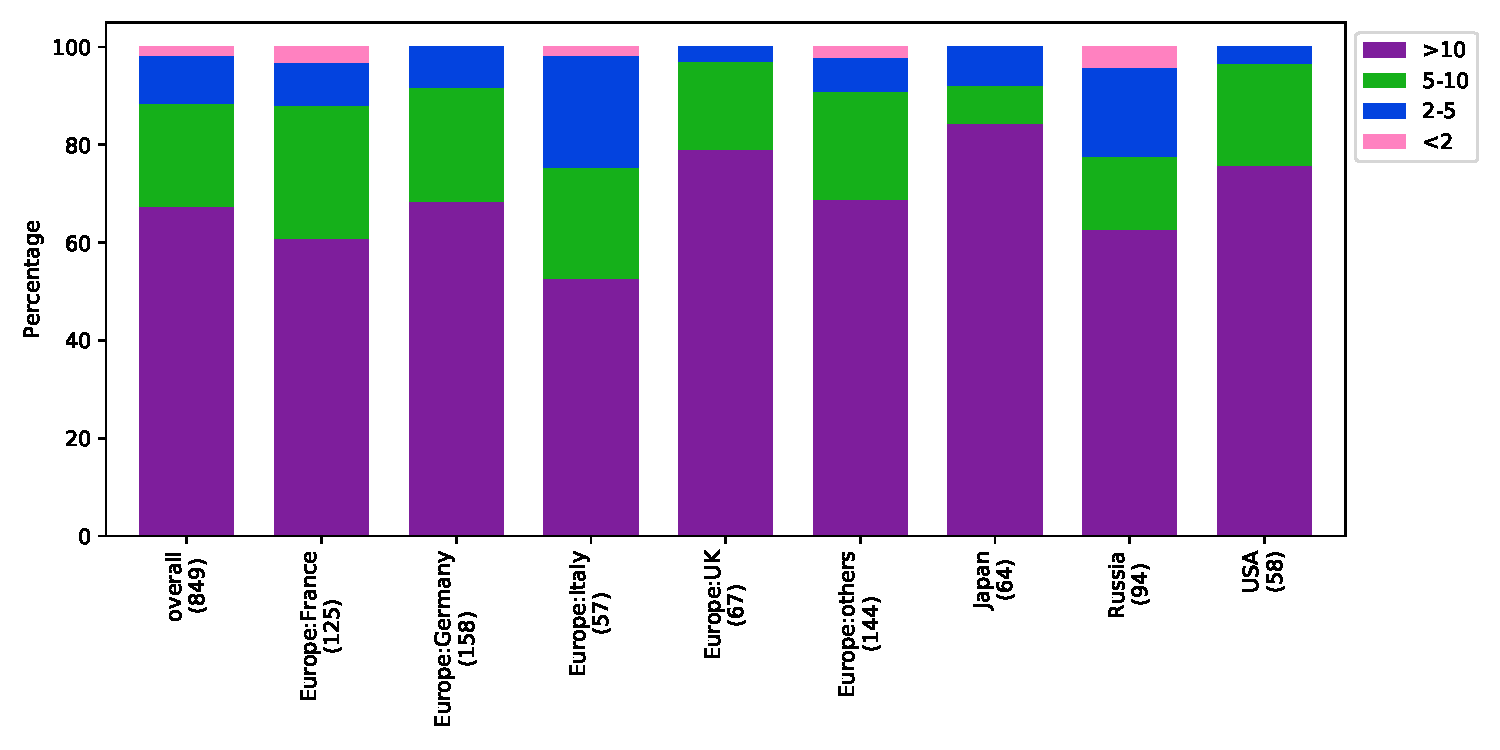
\includegraphics[width=9cm]{../pdfs/Q5.pdf}
  \vspace{-8mm}
\caption{Q5: Programming Experience}
\label{fig:q5}
\end{center}
\end{figure}

\begin{figure}[htb]
\begin{center}
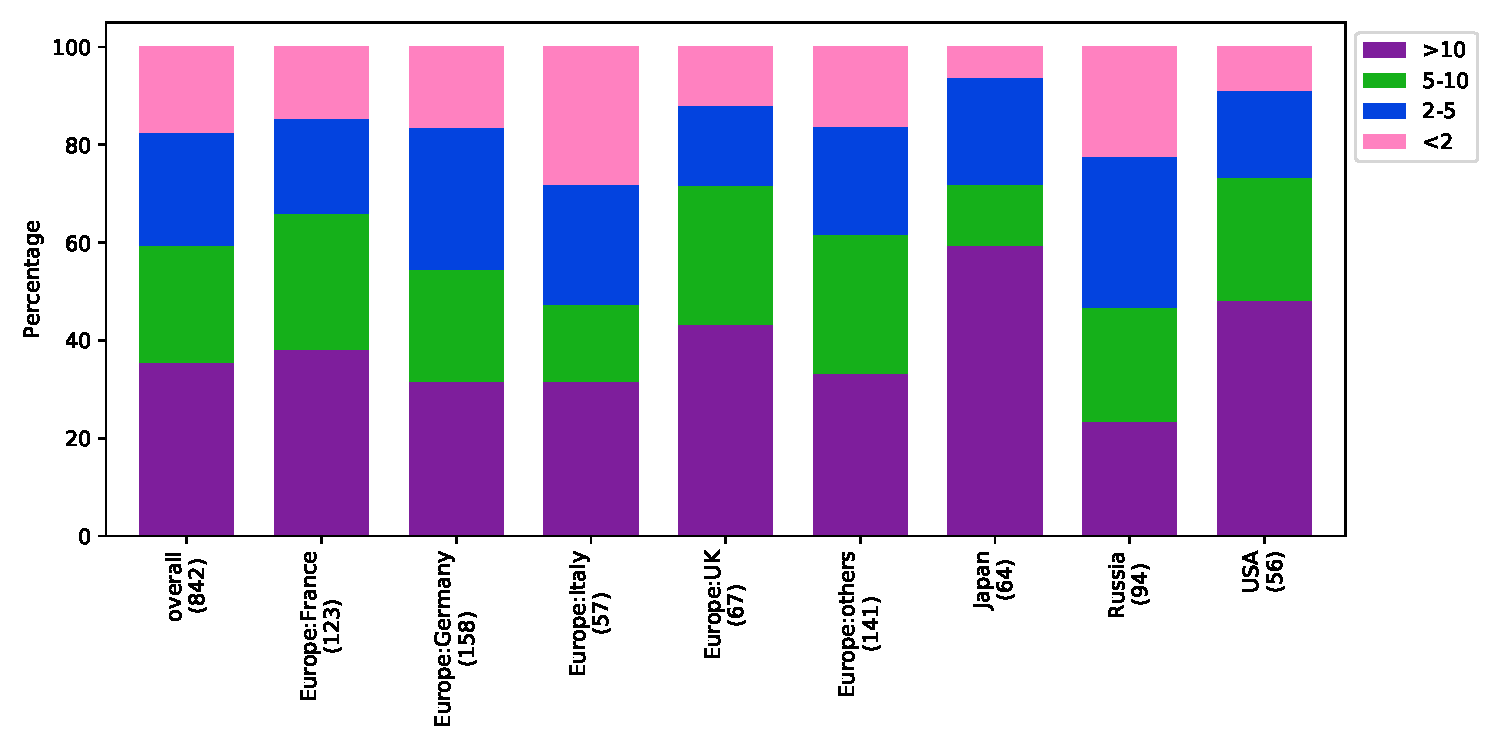
\includegraphics[width=9cm]{../pdfs/Q6.pdf}
  \vspace{-8mm}
\caption{Q6: MPI Experience}
\label{fig:q6}
\end{center}
\end{figure}

It is very interesting that the Japans' percentages of writing MPI and
non-MPI programs more than 10 years are highest among the
others. This looks like the Japanese HPC researchers and programmers
are well-experienced. However, it can also be said that only little young
researchers and programmers are writing MPI programs. Contrastingly
in Germany and Russia cases, novice users, intermediate users, and
experienced users are almost equally distributed.  These look more
ideal than the Japanese case.

\begin{figure}[htb]
\begin{center}
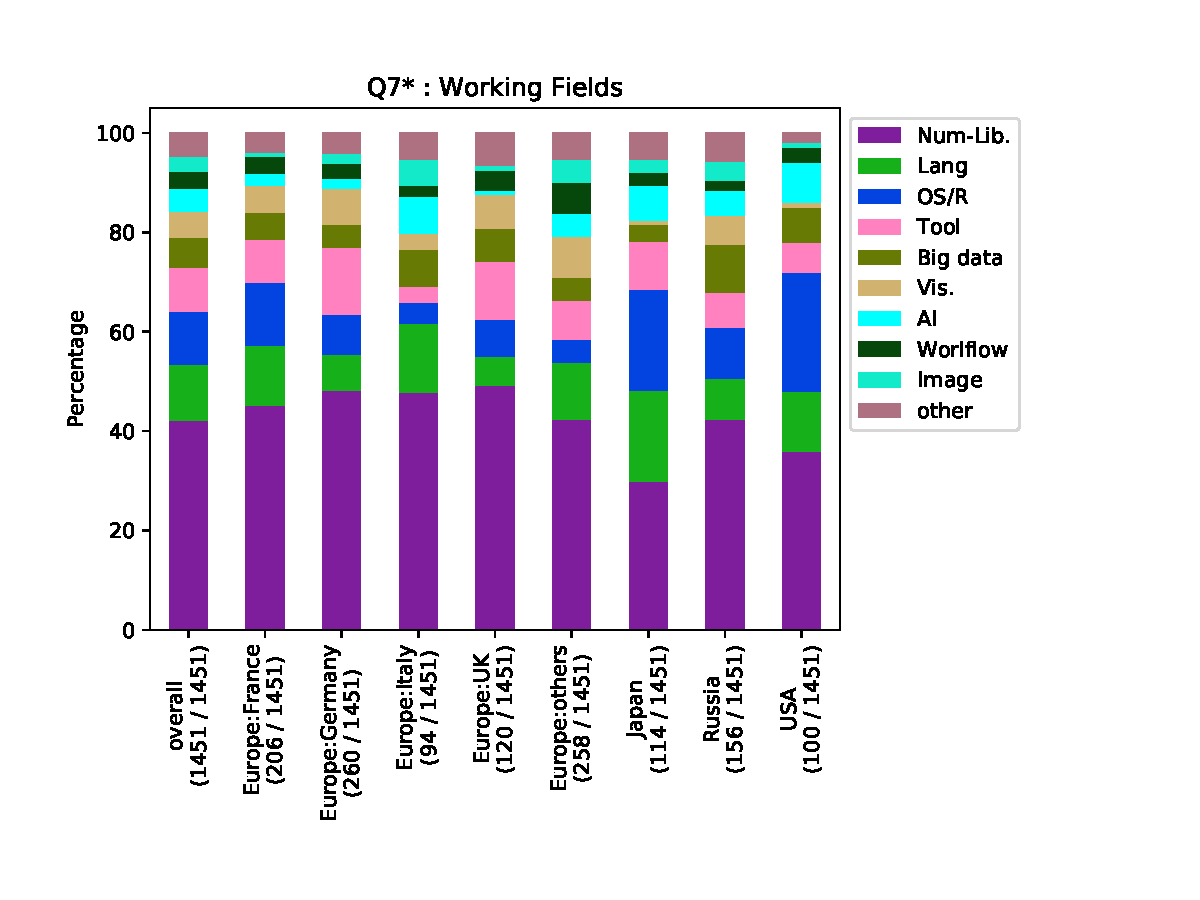
\includegraphics[width=9cm]{../pdfs/Q7.pdf}
  \vspace{-8mm}
\caption{Q7: Field}
\label{fig:q7}
\end{center}
\end{figure}

Figure~\ref{fig:q15} shows the answers asking about the MPI
difficulty. In Japan, the ratios of people having the difficulty for
debugging and tuning are the highest among the other countries. And
the ratios for algorithm selection and domain decomposition, which
are apparently higher levels than the levels of debugging and tuning,
are least among the other countries/regions.

\begin{figure}[htb]
\begin{center}
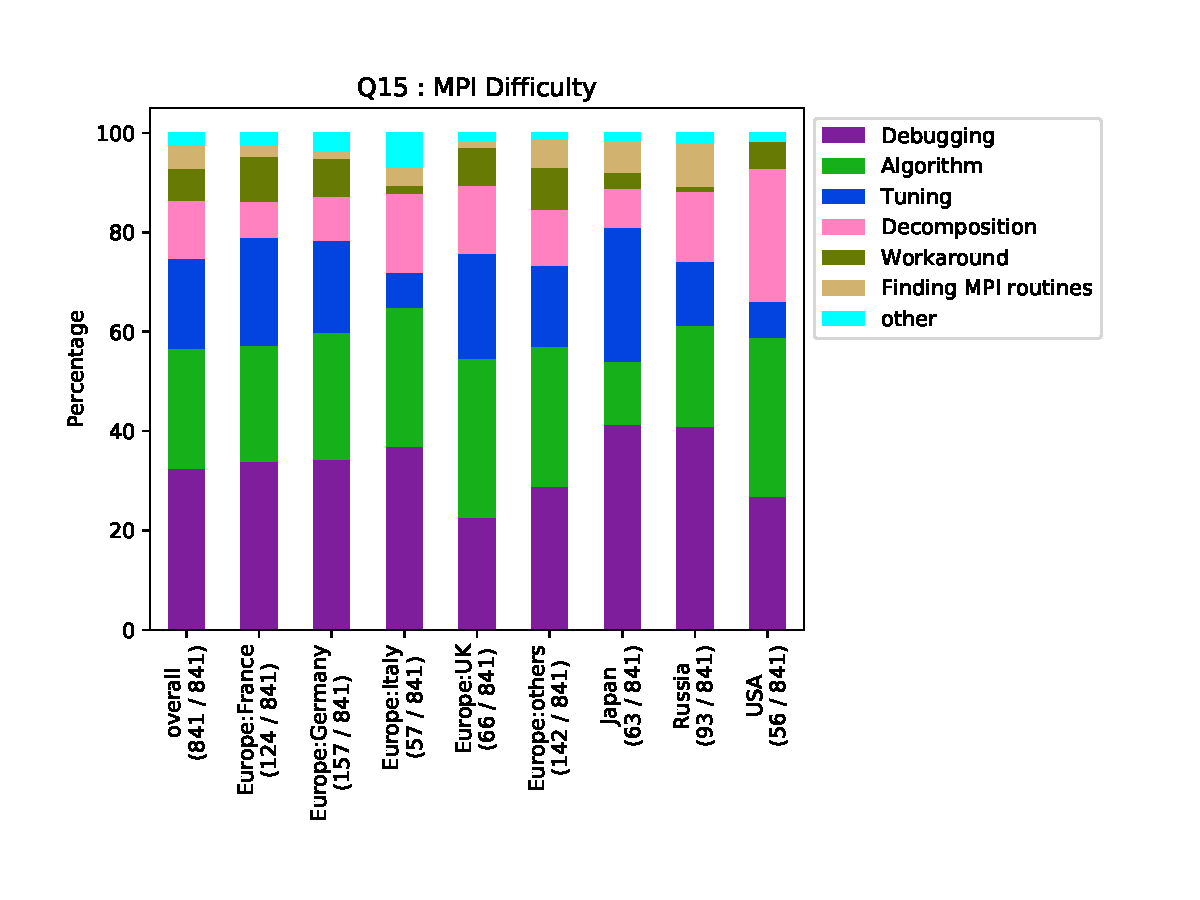
\includegraphics[width=9cm]{../pdfs/Q15.pdf}
  \vspace{-8mm}
\caption{Q15: Difficulty}
\label{fig:q15}
\end{center}
\end{figure}

These results may come from the role of
participants. Figure~\ref{fig:q8} shows the role of 
participants. Unlike the other countries, more Japanese MPI users are
working on research and development of OS and runtime, and less users
are working on tools. This Japan's specificity may affect the result
of Figure~\ref{fig:q5} and \ref{fig:q7}, because the OS and runtime
code are harder to debug and tune than that of applications in many
cases. It is also assumed that algorithm selection and domain
decomposition are the roles of its users. 

\begin{figure}[htb]
\begin{center}
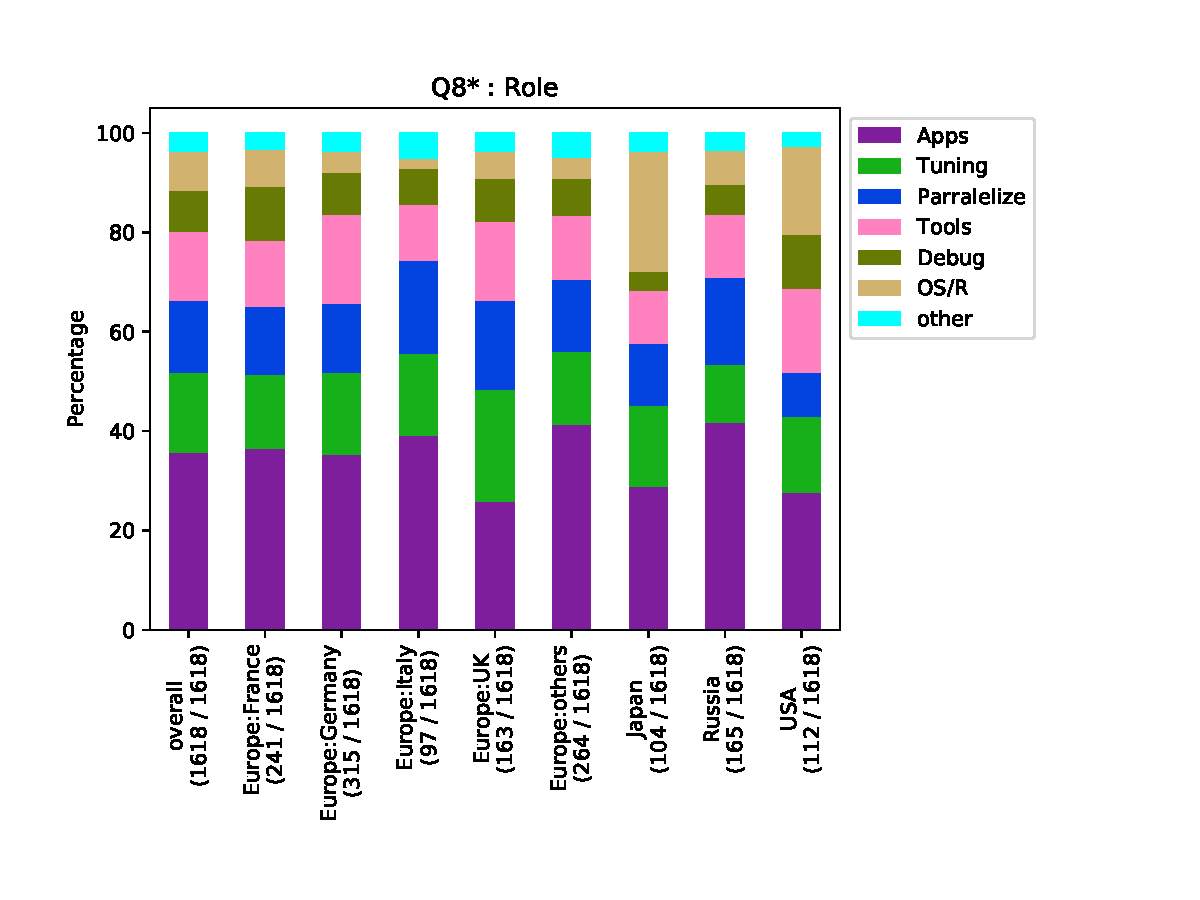
\includegraphics[width=9cm]{../pdfs/Q8.pdf}
\caption{Q8: Role}
\label{fig:q8}
\end{center}
\end{figure}

Figure~\ref{fig:q23} shows the result of asking the room for tuning in
participants' programs. As shown in this figure, Japan has the
lowest ratio of the answer ``My programs are (already) well-tuned.''
At the same time, Japan has the highest ratio of the answer
``Rewriting programs is too hard,'' while they recognize the room for
tuning in their applications. Yes, we agree that rewriting a program
for tuning sometimes requires lots of work; for example, major data
structure changes may affect whole program.

\begin{figure}[htb]
\begin{center}
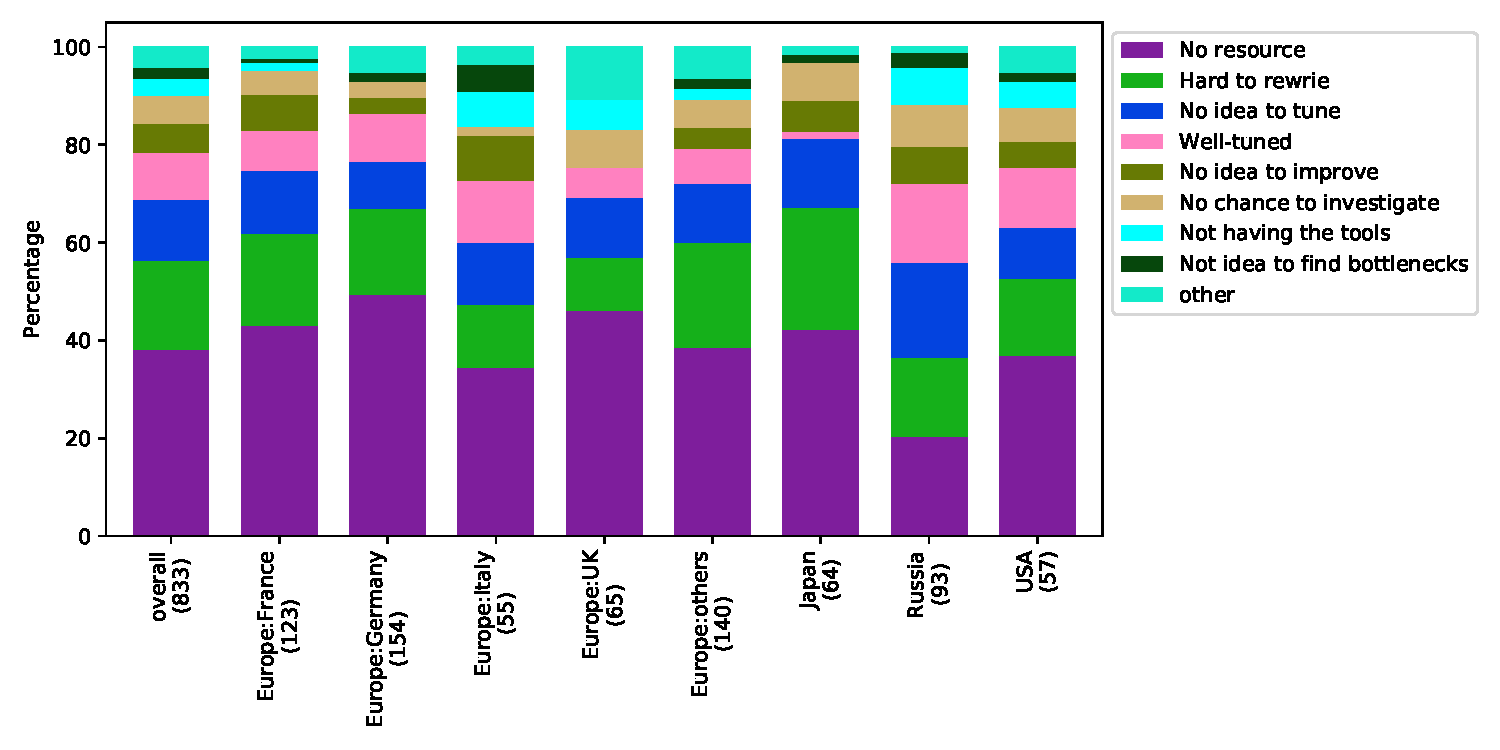
\includegraphics[width=9cm]{../pdfs/Q23.pdf}
\caption{Q23: Room for Tuning}
\label{fig:q23}
\end{center}
\end{figure}

In this question, there is another choice of ``I do not have
enough resource for tuning.'' What is the difference between the
answers of ``rewriting is too hard'' and ``not having enough
resource?'' Considering with the lowest ratio of ``My programs are
well-tuned'' answer, ``rewriting...'' answer sounds like a trouble or
{\it giving up thinking} while the latter one sounds more aggressive.


The cross-tab graphs in this section are the heatmap graphs. The
higher (darker) the value (color) of each cell, the higher the
frequency of the cell. There are nine graphs in this figure, each
graph represents a country or region. All garphs have the same scale.
The lower-right graph is the legend of these graphs serving as a color
bar, too. The numbers in the cells in the legend graph are
percentages. The rows and columns consisting only of the cells less
than 4\% in all countries/regions are omitted to increase readability.

\begin{figure}[htb]
\begin{center}
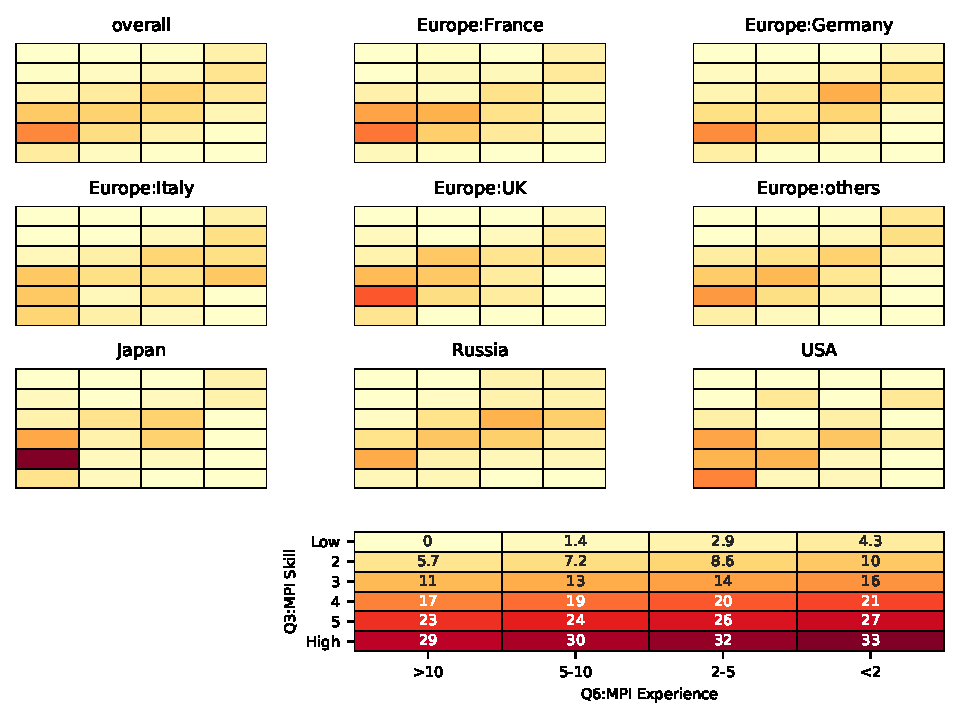
\includegraphics[width=9cm]{../pdfs/Q3-Q6.pdf}
\caption{Q3-Q6: MPI Skill and MPI Experience}
\label{fig:q3-q6}
\end{center}
\end{figure}

Figure~\ref{fig:q3-q6} shows cross-tab graphs between
Q3 (asking MPI skill) and Q18 (asking MPI experience). As shown in
this figure, Japanese answers are concentrated in the cell with the high
MPI skill of 5 (out of 6, larger the number, higher the skill) and
having more than 10 years of MPI experiences. Although the Japan's
Mhigh peak makes the peaks of the others lower and hard to see, the
peaks of the other countries are rather distributed.  

\begin{figure}[htb]
\begin{center}
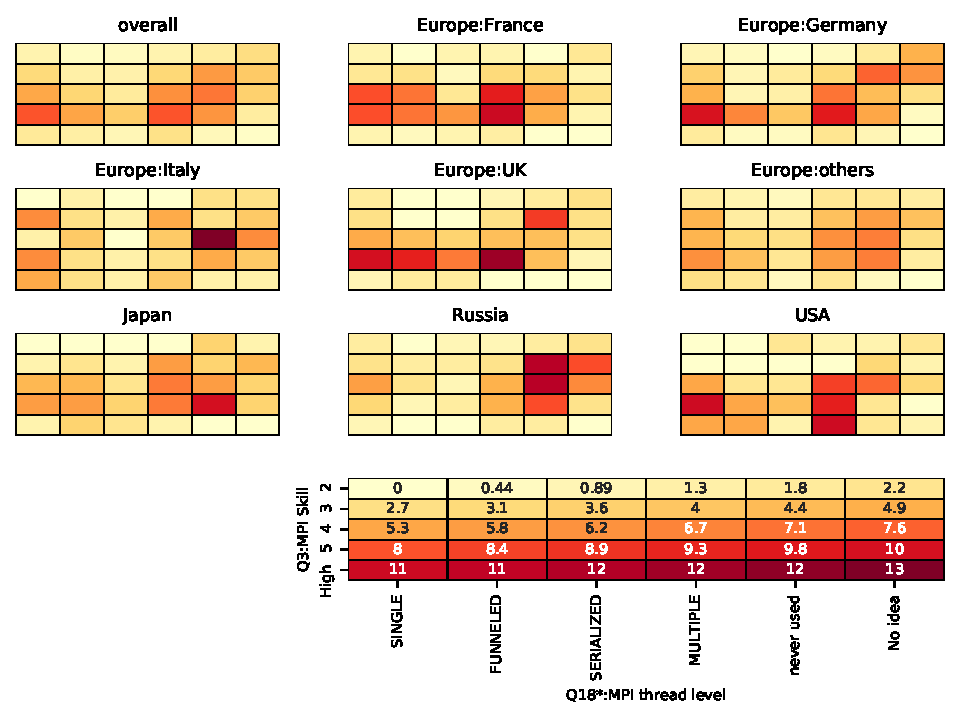
\includegraphics[width=9cm]{../pdfs/Q3-Q18.pdf}
\caption{Q3-Q18: MPI Experience and MPI Thread Level}
\label{fig:q3-q18}
\end{center}
\end{figure}

Figure~\ref{fig:q3-q18} shows the cross-tab graphs between
Q3 (asking MPI skill, again) and Q18 (asking MPI thread
level). There is a peak at 'Never used,' this means that many Japanese
participants do not explicitly call the {\tt MPI\_Init\_thread}
function.  The doubt here is why Japanese MPI {\em experts} do not
call the {\tt MPI\_Init\_thread} function. 
In contrast, in the Russian case, the ratio of ``Never used'' answer
increases when the  MPI skill decreases. In the USA case, the ratio of
using {\tt MPI\_THREAD\_MULTIPLE} increases when the MPI skill goes
up. Those situations are quite reasonable. Thus, the Japanese
specificity comes to the front. 
